\begin{document}
\title{Übungsblatt~2}
\subtitle{Einführung, Dateiverwaltung}
\maketitle

\section*{Lernziele}
\begin{itemize}
	\item Auftretende Probleme bei nicht isolierten Transaktionen
	\item Möglichkeiten, diese Probleme zu erkennen und zu vermeiden
	\item Möglichkeiten zur Recovery unter Verwendung von Logs
\end{itemize}


\section*{Literatur}
\HaerderNintyNine{14}

\ElmasriFive{18, insbes. 18.1}

\GarciaMolinaFirst{18}

\BerensonNintyFive

\section{Fragen zur Vorlesung}

\begin{enumerate}[a)]
	\item Welche möglichen Probleme bei der gleichzeitigen Ausführung von Transaktionen haben Sie in der Vorlesung kennengelernt?

\begin{solution}
\begin{itemize}
	\item Verlorengegangene Änderung (Dirty Write, Lost Update)
	\item Lesen nicht freigegebener Änderungen (Dirty Read)
	\item Inkonsistente Analyse (Non-Repeatable Read)
	\item Phantom-Problem
\end{itemize}
Für die Anomalien im Mehrbenutzerbetrieb gibt man bestimmte Abläufe,
d.\,h.\ Ausführungsreihenfolgen von Operationen verschiedener Transaktionen,
als Muster an.
Beinhaltet ein Ablauf das Muster einer Anomalie,
so sagt man:
Die Anomalie tritt in diesem Ablauf auf.

Leider ist die Definition der Anomalie-Muster umstritten.
Das zeigt sich u.\,a.\ daran, dass viele reale Systeme (z.\,B.\ Oracle, PostgreSQL) nach unserer Definition nicht serialisierbar (und damit möglicherweise nicht korrekt) arbeiten, da sie eine andere Definition verwenden.
Für eine tiefere Beschäftigung mit dieser Tatsache sei der Artikel von Berenson et al.\ empfohlen.
Für diese Veranstaltung ist das aber nicht notwendig.

Da aber eine Definition von Anomalie-Abläufen nötig ist, um über Anomalien sprechen zu können, verwenden wir die Definitionen aus dem Artikel von Berenson et al. (Vorlesungsfolie~\AnomalieDef):

\paragraph{\color{solutioncolor}Dirty Write}
$w_1[x] \ldots w_2[x] \ldots
((c_1 \textrm{ oder } a_1) \textrm{ und } (c_2 \textrm{ oder } a_2)$
in beliebiger Reihenfolge)

Zwei Transaktionen schreiben überschneidend dasselbe Datenelement,
wodurch Inkonsistenzen entstehen können
und das Rücksetzen von Transaktionen erschwert wird.

\paragraph{\color{solutioncolor}Dirty Read}
$w_1[x] \ldots r_2[x] \ldots
((c_1 \textrm{ oder } a_1) \textrm{ und } (c_2 \textrm{ oder } a_2)$
in beliebiger Reihenfolge)

Transaktion~2 hat Daten gelesen, die inkonsistent zu anderen Daten sein können und die eventuell "`nie existiert haben"', da Transaktion~1 abgebrochen werden könnte und damit alle ihre Änderungen rückgängig gemacht werden.

\paragraph{\color{solutioncolor}Non-Repeatable Read}
$r_1[x] \ldots w_2[x] \ldots
((c_1 \textrm{ oder } a_1) \textrm{ und } (c_2 \textrm{ oder } a_2)$
in beliebiger Reihenfolge)

Transaktion~1 sieht, wenn sie erneut liest, einen anderen Wert als zuvor. Dadurch kann es zu inkonsistenten Analysen kommen.

\paragraph{\color{solutioncolor}Phantom-Problem}
$r_1[P] \ldots w_2[y \textrm{ in } P] \ldots
((c_1 \textrm{ oder } a_1) \textrm{ und } (c_2 \textrm{ oder } a_2)$
in beliebiger Reihenfolge);
$P$ steht hier für die Menge der Datenobjekte, die ein Prädikat erfüllen.

Nachdem Transaktion~1 $P$ liest, verändert Transaktion~2 diese Menge durch Einfügen eines geeigneten Tupels, wodurch inkonsistente Analysen entstehen können.
\end{solution}

\begin{note}
Eine Anomalie liegt unabhängig davon vor, ob die Transaktionen mit Abort oder Commit enden, und unabhängig von der Reihenfolge des Endes. Damit die Anomalie vorliegt, dürfen beide Transaktionen aber erst \emph{nach} den anderen Operationen (z.\,B.\ $(r_1[x] w_2[x])$ bei Non-Repeatable Read) enden. Der Ablauf $(r_1[x] c_1[x] w_2[x] a_2[x])$ ist also kein Non-Repeatable Read, der Ablauf $(r_1[x] w_2[x] c_1[x] a_2[x])$ schon.

Das Datenbanksystem kann nicht prüfen, ob eine Anomalie zu einem Problem wird oder nicht, da es nicht weiß, was das Anwendungsprogramm mit den Daten macht. Sobald eine Anomalie vorliegt, besteht aber die Möglichkeit, dass ein Problem, also ein anderes Ergebnis als bei einem seriellen Ablauf, entsteht. Deshalb muss das Datenbanksystem Abläufe mit Anomalien verhindern. Umgekehrt betrachtet muss also in jedem Ablauf, der zu einem Problem führt, eine Anomalie vorliegen.

Beispiel für ein Non-Repeatable Read (und dafür, warum nach Berenson et al.\ kein zweites $(r_1[x])$ gefordert wird), direkt aus Berenson et al.:

x und y seien zwei Kontostände, T1 möchte die Summe der beiden Kontostände ermitteln, T2 nimmt eine Umbuchung von 40 von x auf y vor.

$(r_1[x=50] r_2[x=50] w_2[x=10] r_2[y=50] w_2[y=90] c_2 r_1[y=90] c_1)$

T1 sieht eine Summe von 140 statt der korrekten 100. Die Anomalie ist ein Non-Repeatable Read aufgrund von $(r_1[x=50] \ldots w_2[x=10] \ldots c_2 \ldots c_1)$
Würde Non-Repeatable Read ein zweites $(r_1[x])$ erfordern, würde in dem Ablauf keine Anomalie auftreten.

Zentraler Punkt in Berenson et al., \emph{A Critique of ANSI SQL Isolation Levels} ist folgender:
Einige Anomalien werden durch den SQL-Standard wie folgt definiert:
\begin{enumerate}[i)]
  \item P1 ("`Dirty read"'): SQL-transaction $T_1$ modifies a row. SQL-transaction $T_2$ then reads that row before $T_1$ performs a COMMIT. If $T_1$ then performs a ROLLBACK, $T_2$ will have read a row that was never committed and that may thus be considered to have never existed.

  \item P2 ("`Non-repeatable read"'): SQL-transaction $T_1$ reads a row. SQL-transaction $T_2$ then modifies or deletes that row and performs a COMMIT. If $T_1$ then attempts to reread the row, it may receive the modified value or discover that the row has been deleted.

  \item P3 ("`Phantom"'): SQL-transaction $T_1$ reads the set of rows N that satisfy some $<$search condition$>$. SQL-transaction $T_2$ then executes SQL-statements that generate one or more rows that satisfy the $<$search condition$>$ used by SQL-transaction $T_1$. If SQL-transaction $T_1$ then repeats the initial read with the same $<$search condition$>$, it obtains a different collection of rows.
\end{enumerate}

Dabei ist nun ungeklärt, ob der jeweilige "`If"'-Teil zur Definition der Anomalie gehört oder nur eine Erklärung dessen darstellt, was bei Auftreten der Anomalie passieren kann. Konkret: Muss $T_1$ ein ROLLBACK durchführen, damit ein Dirty Read vorliegt? Oder liegt der bereits durch $w_1(x) r_1(x)$ vor und der "`If $T_1$ \ldots "'-Satz erläutert nur, warum das schlimm sein kann? Genau das ist umstritten. Aber für uns gelten die Definitionen, die oben angegeben sind.
\end{note}

\item Definieren Sie den Begriff "`Serialisierbarkeit"'.

\begin{solution}
Direkt aus den Vorlesungsfolien:
Ein Schedule von Transaktionen ist serialisierbar, wenn er zu irgendeinem seriellen Ablauf der in ihm enthaltenen Transaktionen äquivalent ist.
\end{solution}


\item Seien $T_i$ und $T_j$ beliebige Transaktionen und $H$ und $G$ zwei
  dazugehörige Abläufe. Markieren Sie die Bedingungen, die für alle
  Operationen auf einem beliebigen Datenobjekt $A$ gelten müssen, damit
  zwei Abläufe nach der Definition der Vorlesung "`äquivalent"' sind.
  \nt{Studierende darauf Hinweisen, dass in der Klausur ausgefüllt und nicht gekreuzt wird. Korrekturen mit Korrekturband.}

  \begin{itemize}
    \itemmc   \hspace*{0.45em} $r_i[A] <_H r_j[A] \Leftrightarrow r_i[A] <_G r_j[A]$
    \itemmcsol \hspace*{0.45em} $r_i[A] <_H w_j[A] \Leftrightarrow r_i[A] <_G w_j[A]$
    \itemmcsol \hspace*{0.45em} $w_i[A] <_H r_j[A] \Leftrightarrow w_i[A] <_G r_j[A]$
    \itemmcsol \hspace*{0.45em} $w_i[A] <_H w_j[A] \Leftrightarrow w_i[A] <_G w_j[A]$
  \end{itemize}

\item Geben Sie eine Möglichkeit an, Serialisierbarkeit zu gewährleisten.

\begin{solution}
Serialisierung oder Sperren.
Abhängigkeitsgraphen zählen nicht, da sie zur Prüfung dienen.
Sicherstellen muss man das dann noch auf anderem Wege.
\end{solution}

\begin{note}
Aus didaktischen Gründen lassen wir den Unterschied zwischen Konflikt-Serialisierbarkeit und anderen Serialisierbarkeitsarten aus.
Ersteres ist ein stärkeres Kriterium und wird sowohl durch Abhängigkeitsgraphen als auch durch 2PL gewährleistet.
Wir verbieten also einige Abläufe, die wir eigentlich erlauben könnten.
Grund: Konflikt-Serialisierbarkeit ist leichter zu prüfen.
\end{note}

\end{enumerate}


\section{Fragen zur Vorlesung}
\begin{enumerate}[a)]
	\item Was ist der Vorteil eines B-Baums gegenüber binären Suchbäumen?

	\begin{solution}
	Größerer Fan-Out (Verzweigungsgrad) $\rightarrow$ Grundidee: Blockzugriff ist teuer, also weniger davon machen.

	Das ist auch der Grund, warum ein Knoten gerade so groß wie ein Block ist. Ein Knoten ist die Einheit, in der wir nach der nächsten Verzweigung suchen. Sie sollte komplett zur Verfügung stehen und keine zwischenzeitlichen I/Os verursachen.
	\end{solution}


	\item Was sind die charakteristischen Eigenschaften eines B-Baums?

	\begin{solution}
	Perfekt balanciert (alle Pfade von der Wurzel zu einem Blatt sind gleich lang), jeder innere Knoten hat zwischen $k+1$ und $2k+1$ Nachfolger. Jeder Knoten außer der Wurzel ist mindestens zur Hälfte gefüllt. Die Wurzel ist ein Blatt (dann besteht der Baum nur aus der Wurzel) oder sie hat mindestens 2 Nachfolger.
	\end{solution}


	\item Was unterscheidet den B*-Baum vom B-Baum? Was sind die Vor- und Nachteile?

	\begin{solution}
	Beim B*-Baum werden die Nutzdaten (Satzadresse, oder auch ganzer Satz bei Primärorganisation) nur in den Blättern gespeichert. Das reduziert die Höhe des Baums (durch den höheren Verzweigungsgrad oben) und erlaubt Bereichsanfragen durch Verkettung der Blätter.
	\end{solution}

	\item Zeichnen Sie schematisch den Aufbau eines Blattknotens und eines inneren Knotens eines B*-Baums.

	\begin{solution}

	Innerer Knoten:

		\begin{center}
		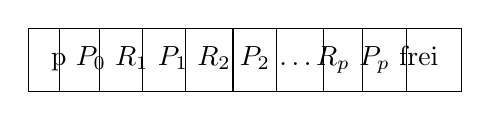
\begin{tikzpicture}

				\node at (2.35, 2.4) {p  $P_{0}$  $R_{1}$  $P_{1}$  $R_{2}$  $P_{2}$  \dots  $R_{p}$  $P_{p}$  frei};

				%Male ausgefülltes Rechteck
				%\fill[fill=lightgray](2.75, 2) rectangle+(0.4, 0.8);

				%Rechteck
				%     links hoehe         rechts hoehe
				\draw (-0.4,2) rectangle +(5.5, 0.8);

				%Senkrechte Striche
				\draw (0, 2) -- (0, 2.8)
							(0.5, 2) -- (0.5, 2.8)
							(1.05, 2) -- (1.05, 2.8)
							(1.6, 2) -- (1.6, 2.8)
							(2.2, 2) -- (2.2, 2.8)
							(2.75, 2) -- (2.75, 2.8)
							(3.35, 2) -- (3.35, 2.8)
							(3.85, 2) -- (3.85, 2.8)
							(4.4, 2) -- (4.4, 2.8)
							;

		\end{tikzpicture}
		\end{center}



	Wobei $P_{i}$ ein Zeiger auf einen weiteren inneren oder Blattknoten und $R_{i}$ ein Referenzschlüssel ist. p ist die Anzahl der Einträge. Es gilt: $k \leq p \leq 2 k$

	Blattknoten:

		\begin{center}
		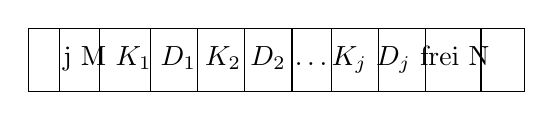
\begin{tikzpicture}

				\node at (2.35, 2.4) {j  M  $K_{1}$  $D_{1}$  $K_{2}$  $D_{2}$  \dots  $K_{j}$  $D_{j}$  frei   N};

				%Rechteck
				%     links hoehe         rechts hoehe
				\draw (-0.8,2) rectangle +(6.3, 0.8);

				%Senkrechte Striche
				\draw (-0.4, 2) -- (-0.4, 2.8)
							(0.1, 2) -- (0.1, 2.8)
							(0.75, 2) -- (0.75, 2.8)
							(1.35, 2) -- (1.35, 2.8)
							(1.95, 2) -- (1.95, 2.8)
							(2.55, 2) -- (2.55, 2.8)
							(3.05, 2) -- (3.05, 2.8)
							(3.65, 2) -- (3.65, 2.8)
							(4.25, 2) -- (4.25, 2.8)
							(4.95, 2) -- (4.95, 2.8)
							;

		\end{tikzpicture}
		\end{center}
	Wobei $K_{i}$ ein Referenzschlüssel ist und $D_{i}$ die Nutzdaten zum Schlüssel $K_{i}$. j ist die Anzahl der Einträge. Es gilt: $k^* \leq j \leq 2 k^*$. $M$ ist der Zeiger auf den vorherigen und $N$ der Zeiger auf den nächsten Blattknoten.

	\end{solution}

	\item Ist in einem B*-Baum jeder Schlüsselwert, der in einem inneren Knoten gespeichert ist, auch in einem Blattknoten vorhanden?

	\begin{solution}
		Nein. Es kann zum Beispiel durch Löschen eines Eintrags in einem Blattknoten die Situation entstehen,
		dass in einem inneren Knoten ein Referenzschlüssel vorkommt, der in keinem Blattknoten mehr enthalten ist. \\
		Selbstverständlich bleibt jedoch die Semantik erhalten, dass vor einem Referenzschlüssel nur Einträge mit niedrigeren
		oder gleichen Schlüsselwerten und nach dem Referenzschlüssel nur Einträge mit höheren Schlüsselwerten vorkommen.
	\end{solution}

	\item Welche Möglichkeiten fallen Ihnen ein, um Einträge wieder aus einem Index zu entfernen?

	\begin{solution}
		Die Einträge können direkt aus dem Index gelöscht werden. Das erfordert jedoch je nach Index und verwendeter Implementierung eine z.\,T. sehr aufwendige Reorganisation. Löschen in Hashtabellen mit quadratischem Sondieren ist komplex bis unmöglich, ohne kompletten Neuaufbau des Indexes. Löschen aus einem B-Baum kann eine ganze Reihe von Unterläufen und im Laufe der Unterlaufbehandlung wieder Überläufen erzeugen.

		Eine andere Möglichkeit ist, die Einträge als "`gelöscht"' zu markieren, ohne sie tatsächlich zu entfernen. So macht es z.\,B. auch Oracle in seinen B-Baum-Indizes. Hierdurch geht das Löschen sehr schnell. Der Speicherbedarf ist durch die gelöschten Elemente aber höher und kann je nach Struktur auch die Kosten für Einfügen und Suchen erhöhen. Der zusätzliche Aufwand hierfür ist abhängig von der Indeximplementierung und der Zahl der Löschvorgänge.

		Als Kompromisslösung bietet es sich an, Einträge als gelöscht zu markieren und ab einem gewissen Punkt, zum Beispiel einem bestimmten Prozentsatz von Platzhaltern in Bezug zur Gesamtzahl an Einträgen, die Tabelle neu aufzubauen. Bei Oracle stehen Informationen über den Zustand des Indexes bereit und der Administrator entscheidet darüber, wann ein Index neu aufgebaut werden soll.
	\end{solution}

	\item Welche Daten müssen und welche können in einem Index gespeichert werden?

	\begin{solution}
		Der Indexwert (Schlüssel) muss immer gespeichert werden. Was zusätzlich noch gespeichert wird, hängt davon ab, für was der Index benutzt werden soll:

		\begin{description}
			\item[Keine weiteren Informationen] Bereits nichts weiter als nur den Indexwert zu speichern kann Anfragen unterstützen, wenn oft überprüft werden soll, ob ein Schlüsselwert vorhanden ist, aber der zugehörige Satz nicht weiter interessiert (z.\,B. für Unique-Attribute oder zur Unterstützung einer \texttt{contains}-Funktion).
			\item[TID] Zusätzlich wird die Satzadresse des Satzes gespeichert. Dadurch wird der Schlüsselzugriff auf den Satz ermöglicht.
			\item[(TID +) Teil eines Satzes] Zusätzlich zum Schlüsselwert und der Satzadresse werden noch ein oder mehrere Felder gespeichert. Das erfordert natürlich einen höheren Platzbedarf, kann aber sinnvoll sein, wenn häufig Anfragen
			gestellt werden, die den Schlüssel und bestimmte Felder benutzen. Man spart sich den Zugriff über die Satzadresse, wenn die benötigten Felder bereits im Index stehen.
			Durch das Weglassen der TID erhält man eine Datenstruktur, die nur bei Anfragen auf die in der Struktur abgelegten Teile verwendet werden kann. Andernfalls ist der Index für diese Anfrage nicht benutzbar.
			\item[Ganzer Satz] Der ganze Satz wird im Index gespeichert. (Primärorganisation)
			\item[Mehrere TIDs, Teile von Sätzen, Sätze] Bei einem Index über ein nicht-eindeutiges Attribut kann es zu einem Schlüsselwert mehrere Tupel geben. Diese werden dann alle zusätzlich zum Schlüsselwert abgelegt. Hierfür sind, genauso wie für die Ablage variabel langer Sätze in einem Index, angepasste Index-Algorithmen notwendig, die variabel lange Einträge unterstützen.
			\item[TIDs, Teile von Sätzen, Sätze anderer Relationen] Bei einem Index über einen Primärschlüssel können sowohl die TIDs der beinhaltenden Relation als auch die TID der referenzierenden Relation mit Fremdschlüssel gespeichert werden, um den Join zu erleichtern. Natürlich lassen sich bei dieser Vorgehensweise alle anderen Optionen (Teile des Satzes, Ganzer Satz) genauso anwenden.
		\end{description}

		%Indexwert muss, TID, ganzes Tupel, Teil eines Tupels kann. Nur Indexwert könnte auch sinnvoll sein, wenn nur auf Vorhandensein geprüft werden soll.
	\end{solution}
\end{enumerate}

\begin{note}
Darauf hinweisen, dass B-Bäume der Standard bei der Implementierung von Indizes sind.

Außerdem darauf hinweisen, dass die Bezeichnung B$^\text{+}$-Baum dasselbe Konzept
meint, das wir als B*-Baum bezeichnen.
\end{note}




\section{\normaltxt{Bestimmung der }Zugriffslatenzen bei wahlfreiem oder sequentiellem Zugriff}

\subsection{Festplatte}
\label{ZugriffFestplatten}
Stellen Sie sich vor, Sie haben eine Festplatte mit folgenden Leistungsdaten:
\beamertxt{
	\paragraph{Plattenlaufwerk Seagate Ironwolf Pro 18 TB (ST18000NE0000)}
	\begin{itemize}
		\item 480.000 Zylinder
		\item 18 Spuren pro Zylinder
		\item 4064 Sektoren pro Spur
		\item 512 Byte pro Sektor
		\item 7200 RPM
		\item Positionierungszeit (Seek-Zeit) Annahme: 4 ms
		\item Track-to-Track-Zeit Annahme: 0,2ms
		\item Kosten 550€ (10/2021)
	\end{itemize}
	\pagebreak}
\paragraph{Plattenlaufwerk Seagate Ironwolf Pro 18 TB (ST18000NE0000)}
\begin{itemize}
	\item 480.000 Zylinder
	\item 18 Spuren pro Zylinder
	\item 4064 Sektoren pro Spur
	\item 512 Byte pro Sektor
	\item 7200 RPM
	\item Positionierungszeit (Seek-Zeit) Annahme: 4 ms
	\item Track-to-Track-Zeit Annahme: 0,2ms
	\item Kosten 550€ (10/2021)
\end{itemize}

\paragraph{Aufgabe}
\begin{enumerate}[a)]
	\item Wie lange benötigen Sie im Mittel, um
	\label{ZugriffFestplattenDauern}

	\begin{enumerate}[i)]
		\item 10.000 aufeinander folgende Blöcke (4KiB) zu lesen?

\begin{solution}
	\begin{note}
		Evtl vorher berechnen:
		\begin{itemize}
			\item Zeit pro Umdrehung (60s/7200) = 8,33ms
			\item Blöcke pro Spur = 4064/8 = 508
		\end{itemize}
	\end{note}
	Zur Berechnung benötigt man neben den obigen Zeitangaben noch die mittlere Zugriffszeit $T_{Zugriff}$.
	Diese setzt sich zusammen aus der Seek-Zeit $T_{Seek}$ und der Rotationslatenzzeit $T_{Rotationslatenz}$, also der Zeit, die anfällt, wenn der Schreib-/Lesekopf schon über der richtigen Spur ist, bis die Blöcke mit den Zieldaten unter dem S/L-Kopf sind.
	Wir nehmen für $T_{Rotationslatenz}$ die Hälfte der Dauer für eine Umdrehung an.
	Daraus folgt:
	\begin{align*}
	T_{Zugriff} &= T_{Seek} + T_{Rotationslatenz}\\
	&= 4ms + 0,5\cdot 60/7200 s  = 4ms + 4,16ms\\
	&= 8,16ms
	\end{align*}
	Im Anschluss kann die ganze Spur in $T_{Rotation}$ gelesen werden.
	Doch wie viele Spuren müssen gelesen werden?
	\begin{align*}
		\textit{Blöcke pro Spur} &= \textit{Sektoren pro Spur} / \textit{Sektoren pro Block} = 4064/8 = 508\\ 
		\textit{Anzahl an Spuren} &= \textit{Anzahl an Blöcken} / \textit{Blöcke pro Spur}\\
		&= 10.000 / 508 \approx 19,69
	\end{align*}
	Damit müssen 18 bis 19 volle Spuren und bis zu zwei Spuren im Anteil gelesen werden.
	Im einfachsten Fall haben wir eine erste Spur, 18 volle Spuren und eine zusätzliche Spur für den Rest.
	Um zwischen 2 benachbarten Spuren zu wechseln fällt keine ganze $T_{Seek}$ an, sondern lediglich eine $T_{Track2Track}$.
	Die beiden unvollständigen Spuren haben in Summe $10.000 - 18*508 = 856$ Blöcke.
	Damit erhalten wir:
	\begin{align*}
		T_{10.000} &= T_{erste Spur} + 18\cdot T_{ganze Zusätzliche Spur Lesen} + T_{letzte Spur}\\
		&= T_{Zugriff} + T_{Lesen Erste Spur}\\
		&+ 18 (T_{Track2Track} + T_{Rotationslatenz} + T_{Rotation})\\
		&+ T_{Track2Track} + T_{Rotationslatenz} + T_{Lesen Letzte Spur}\\
		&= T_{Zugriff} + T_{Lesen Erste Spur} + T_{Lesen Letzte Spur}\\
		&+ 18 (T_{Track2Track} + T_{Rotationslatenz} + T_{Rotation})\\
		&+ T_{Track2Track} + T_{Rotationslatenz}\\
		&= 8,16ms + 856/508 \cdot 8,33 ms\\
		&+ 18 \cdot (0,2ms + 4,16ms + 8,33ms)\\
		&+ 0,2ms + 4,16ms\\
		&\approx 22,2ms + 228,4ms + 4,4ms = 255ms
	\end{align*}
	Die 856 Blöcke können sich jedoch auch auf drei Spuren verteilen.
	\nt{x, 508, y}
	Hier fallen dann zusätzlich noch eine $T_{Track2Track}$ und eine $T_{Rotationslatenz}$ an.
	\begin{align*}
		T_{10.000} &= 255ms + 0.2ms + 4,16ms \approx 259ms
	\end{align*}
\end{solution}


		\item 10.000 irgendwo über die Platte verstreute Blöcke (4KiB) zu lesen?
		Gehen Sie davon aus, dass die Blöcke völlig zufällig verteilt sind.

		\begin{solution}
		Wir gehen in der Musterlösung vom Worst Case aus (= jeder der 10.000 gesuchten Blöcke liegt auf einer anderen zufälligen Spur, was bei 480.000 Spuren nicht unwahrscheinlich ist), d.h. für jeden Block muss $TZugriff$ aufgewendet werden.
		Die Lesezeit für einen Block pro Spur beträgt $1/508$ einer Umdrehung, das ist vernachlässigbar klein.
		Dauer insgesamt: 
		\begin{align*}
			T &= 10000 \cdot ( TZugriff + vernachlaessigbare Lesezeit)\\
			&= 10000 \cdot 8,16ms = 81,6s
		\end{align*}
		\end{solution}

		\begin{note}
		Vielleicht kommt jemand auf die Idee, dass ja rein zufällig zwei Blöcke auf dem gleichen Zylinder liegen.
		Das Geburtstagsparadoxon legt das Nahe.
		Bei insgesamt 10000 Blöcken auf über 480.000 Zylindern (*18 Spuren) liegt die wslkt zwar $99,7\% $, jedoch machen bei 10000 Zugriffen eine Hand voll eingesparte Zugriffe auch keinen allzu großen Unterschied.
		\end{note}

	\end{enumerate}


	\item Was sind die Vorteile beziehungsweise Nachteile von sehr kleinen und sehr großen Blockgrößen innerhalb eines Dateisystems?

	\begin{solution}
	\paragraph{I/O-Operationen}
	Kleine Blockgrößen haben den Nachteil, dass sehr viele I/O-Operationen notwendig (teuer) sind, was bei großen Blockgrößen deutlich weniger wird.
	Außerdem ist der Verwaltungsaufwand bei kleinen Blöcken größer.
	Dafür ist die Platzverschwendung pro Block nicht so groß.

	\paragraph{Speicherplatz}
	Große Blöcke können Speicherplatzverschwendung sein, da man immer einen ganzen Block allokieren muss.
	Wenn z.B. eine Relation sehr klein ist, nutzt sie nicht den ganzen Block aus.
	Umgekehrt bleibt je Block aber im Mittel der Platz für einen halben Satz ungenutzt.
	Somit verschwenden wir bei kleinen Blöcken weniger Platz.
	Das sehen wir aber erst in der nächsten Übung.
	\end{solution}
\end{enumerate}

\subsection{Flash-Speicher}
Seit einigen Jahren werden zunehmend Solid State Disks (SSDs) als Festplattenersatz verwendet.
Diese verwenden Flash-Speicher als Speichermedium.
Die Funktionsweise von Festplatten und SSDs unterscheiden sich deutlich, so dass ein direkter Vergleich schwierig ist.
Weitere Infos zu SSDs können Sie in diesem Blogbeitrag nachlesen: \href{http://databasearchitects.blogspot.com/2021/06/what-every-programmer-should-know-about.html}{databasearchitects.blogspot.com/2021/06/what-every-programmer-should-know-about.html}

Vereinfacht nehmen wir folgende Werte an:

\paragraph{SSD Seagate FireCuda 530 4TB (ZP4000GM30013)}
\begin{itemize}
	\item Random Read (Parallel): 1.000.000 IOPS\normaltxt{ (Input / Output Operations Per Second)}, 4KiB Einheiten
	\item Sequential Read: 7300 MB/s, 128 KiB Einheiten
	\item Leselatenz Annahme: 80µs
	\item Kosten 890€ (10/2021)
	\item Keine Einteilung in Spuren oder Zylinder.
	Die 4KB Einheiten haben quasi eine fortlaufende Blocknummer.
\end{itemize}

\paragraph{Aufgabe}
\begin{enumerate}[a)]
	\item Bestimmen Sie die Lesedauern aus \ref{ZugriffFestplatten} \ref{ZugriffFestplattenDauern}) für die SSD.

	\begin{solution}
	\begin{enumerate}[i)]
		\item Für 10.000 Blöcke der Größe 4KiB benötigen wir $10.000/(128/4) = 312,5$ also 313 bis 314 Einheiten.
		Wie lange dauert es, eine Einheit zu lesen?
		\begin{align*}
			T_{SequenzielleEinheit} &= 128KiB/7300 MB/s\\
			&= (128 \cdot 1024) /(7300 \cdot 1000\cdot 1000) s  \\
			&\approx 18 \mu s
		\end{align*}
		Damit erhalten wir im schlechtesten Fall $18\mu s \cdot 314 = 5,6ms$
		\item Da über jeden NAND-Channel unabhängig zugegriffen werden kann, muss hier der parallele Zugriff vom sequentiellen unterscheiden werden.
		\begin{description}
			\item[parallel] Beim lesen von 10.000 Blöcken benötigt die SSD jeweils eine IOP.
			Damit $10.000/1.000.000 s = 1/100 s = 10 ms$
			\item[sequentiel] Wenn die Blöcke nur einer nach dem anderen zugegriffen werden können, benötigt jeder Block die Leselatenz.
			Damit $10.000\cdot 80\mu s = 800 ms$
		\end{description}
	\end{enumerate}
	\end{solution}

	\item Bestimmen Sie die Kosten für die genannten Datenspeicher in $\geneuro/GB$.
	
	\begin{solution}
		\begin{description}
			\item[HDD] $550\geneuro / 18TB = 550 / (1000*18) \cdot \geneuro/GB \approx 0,03 \geneuro/GB$
			\item[SSD] $890\geneuro / 4TB = 890 /(1000*2) \cdot \geneuro/GB \approx 0,22 \geneuro/GB$
		\end{description}
	Wie Sie erkennen können ist SSD-Speicher etwa um eine Größeneinheit teurer als HDD-Speicher.
	\end{solution}


	\item Wie bereits erwähnt, sind SSDs nicht in Spuren und Zylinder eingeteilt.
	Wie könnte eine einheitliche Schnittstelle aussehen, mit der man Blöcke sowohl von Festplatten als auch von SSDs lesen kann?

	\begin{solution}
	Als gemeinsame Schnittstelle kann man auf jedes Gerät über die Blocknummer zugreifen.
	Das tut man mit LBA (Logical Block Adressing) auch seit über 20 Jahren (Win98 ist zwar noch auf 128\,GB beschränkt, aber schon mit LBA).

	Das ist schon eine Abstraktion: Wir müssen nicht mehr das physische Layout der Daten auf einer Platte kennen; wenn wir die Größe eines Gerätes kennen, können wir alle Blöcke adressieren.
	Diese Abstraktion war auch notwendig, da neuere Platten eine unterschiedliche Anzahl von Blöcken je Spur haben können.
	Gleiches gilt für CDs (constant linear velocity vs. constant angular velocity).
	\end{solution}
\end{enumerate}


\section{Dateiverwaltung}
Welche Operationen müssen in welcher Reihenfolge ausgeführt werden um einen Block einer (blockorientierten) Datei zu lesen?

\begin{enumerate}[\alph{enumi})]
\item Beim öffnen der Datei.
\begin{solution}
\begin{enumerate}
	\item Master File Table bzw. Dateikatalog von dem Laufwerk über die Gerätesteuerung lesen.
	Dieser Dateikatalog liegt an einer fest definierten Stelle auf dem Laufwerk.
	\item Solange die angeforderte Datei nicht gefunden wurde, gehe die Hierarchie des Dateikatalogs durch.
	Dies ist abhängig vom Dateisystem (vgl. Vorlesungsfolien~\Katalogeintraege~und SP2).
	\item Überprüfe ob die Zugriffsrechte des Benutzers mit der angeforderten Zugriffsart übereinstimmen.
	\item Lege den Dateikontrollblock für die Datei an.
\end{enumerate}
\end{solution}
\item Beim lesen aus der geöffneten Datei.
\begin{solution}
\begin{enumerate}
	\item Lese aus dem Dateikontrollblock für die Datei die Referenz zum geforderten Block.
	\item Fordere über die Gerätesteuerung den gewünschten Block an.
	\item Die Gerätesteuerung setzt die Blocknummer in den entsprechenden Zugriffsbefehl für den Hintergrundspeicher um und liefert den Block zurück.
	Bei einer HDD beinhaltet dies die Umwandlung der Blocknummer in Slot, Zylinder und Spur.
\end{enumerate}
\end{solution}
\end{enumerate}


\begin{deeper}
\section{Dateizugriff}
Schreiben Sie im Pseudocode die Operation, die einen Block aus einer Datei liest.
Der Dateikatalog soll als Extent-Tabelle gemäß Folie~\KatalogeintraegeVier~im Anhang realisiert sein.
Die Datei kann als bereits geöffnet angenommen werden.
Die Kommunikation mit der Festplatte sei über die Funktion \texttt{readBlock(int CylinderNo, int TrackNo, int SlotNo, ByteBuffer bb)} der Klasse \texttt{Device} zu gestalten.
Die Signatur der Methode \texttt{read} is Folgende: \texttt{void read(int BlockNo, ByteBuffer bb) throws IOException{}}.

\cprotEnv
\begin{note}
\begin{lstlisting}[]
/* Operation
 * int BlockFile::read ( int BlockNo, char *BlockBuffer )
 * wie auf Folie(*@~\textit{\SchreibUndLese}@*)
 */
void read(int BlockNo, ByteBuffer bb) throws IOException {
/* Lesen der Extent-Tabelle auf dem Katalog-Eintrag der
 * (bereits geöffneten) Datei:
 * Extent[i] (Slot-Adresse; AnzSlots)
 * AnzSlots = Zahl der von dieser Adresse an
 * sequenziell belegten Slots
 */
int LocalBlockNo = BlockNo; bool found=false;
// Finde passenden Extent
for(int i = 0; i < Extent.length; i++) {
  if(LocalBlockNo > Extent[i].AnzSlots ) {
    LocalBlockNo -= Extent[i].AnzSlots;
  } else {found=true; break;}
}
if(!found) throw new IOException();
// Startkoordinaten des Extents
int CylinderNo = Extent[i].Slot-Adresse.Zylinder;
int TrackNo = Extent[i].Slot-Adresse.Spur;
int SlotNo = Extent[i].Slot-Adresse.Slot;
// Bewege Koordinaten entsprechend weiter
SlotNo += LocalBlockNo;
/* Überlaufbehandlung: */
while(SlotNo > SlotsPerTrack) {
  SlotNo -= SlotsPerTrack; TrackNo++;
}
while(TrackNo > TracksPerCylinder) {
  TrackNo -= TracksPerCylinder; CylinderNo++;
}
if(CylinderNo > MaxCylinder) throw new IOException();
int Status = Device.readBlock(CylinderNo, TrackNo, SlotNo, bb )
if (Status != 0)  throw new IOException();
return
}
\end{lstlisting}
\end{note}

\end{deeper}

\section{Zugriffsbeschleunigung}
Überlegen Sie sich einige Ideen, wie die Zugriffszeiten auf externe (Online-)Spei\-cher\-me\-di\-en generell verkürzt werden können.

\begin{solution}
\begin{itemize}
	\item Daten gemäß Zylinder organisieren

	Die "`Seek"'-Zeit macht ca. 50\,\% der mittleren Blockzugriffszeit aus. Durch die Platzierung von logisch zusammen gehörenden Daten, deren Kapazität größer als die einer Spur ist, auf dem gleichen Zylinder fällt die "`Seek"'-Zeit beim Lesen im besten Fall nur einmal an.


	\item Verwendung mehrerer Festplatten -- im weitesten Sinne RAID

	Hier gibt es zwei Möglichkeiten:
	\begin{enumerate}
		\item Auf den Platten stehen die gleichen Daten (Spiegelung, Mirroring).
		\item Die verschiedenen Platten enthalten unterschiedliche Daten.
	\end{enumerate}
	In beiden Varianten können sich die Köpfe der Platten unabhängig voneinander bewegen. 	Daher kann man insgesamt mehr seek-Operationen durchführen und außerdem parallel lesen (Durchsatz!).
	In a) klappt das immer, in b) nur dann, wenn die benötigten Daten auf unterschiedlichen 	Platten liegen. Außerdem bietet a) Datensicherheit zum Preis von verschwendetem 	Speicherplatz.
	Das Schreiben kann in b) schneller werden (analog dem Lesen), in a) nicht, da die Daten 	auf alle Platten gleichzeitig geschrieben werden müssen und man nicht parallel 	unterschiedliche Operationen ausführen kann.
Voraussetzung ist natürlich, dass der Disk-Controller dafür ausgelegt ist und Hauptspeicher und Datenbus mit den höheren Transferraten klar kommen.


	\item Scheduling mit Elevator-Algorithmus

	Will man mehrere Zugriffe tätigen, so kann man das evtl. in einer günstigeren Reihenfolge als der angegebenen machen. Eine günstige Reihenfolge ist eine, die die Kopfbewegungen minimiert. Dazu gibt es z.\,B. den sog. Elevator-Algorithmus: man behält die Richtung der Kopfbewegung solange bei, bis in dieser Richtung keine weiteren Aufträge vorliegen. Dabei bearbeitet man immer den nächstgelegenen Auftrag als nächstes. Das tun Festplatten heute schon selbständig. Das Betriebssystem auch.


	\item Prefetching

	Lesen: Wenn man voraussagen kann, welche Blöcke in naher Zukunft gebraucht werden, kann man sie früh (oder. während man sie sowieso passiert) in den Hauptspeicher laden.
	Das funktioniert natürlich nur, wenn die Platte nicht dauerhaft unter Last steht und man 	"`freie Zeit"' zum Prefetching verwenden kann. Für das Lesen "`während man sie sowieso passiert"' braucht man natürlich keine freie Zeit.

	Schreiben: analog

	Sonstige Arten von Pufferung (Caches) zählen wir hier noch nicht, da sie nicht direkt die Zugriffszeiten verringern, sondern gleich die Zugriffe vermeiden.

	\item Komprimierung

	Wenn die Daten auf der Platte effektiv komprimiert wurden, belegen sie weniger Blöcke und können daher schneller in den Hauptspeicher geladen werden. Siehe dazu später auch C-Store (Vorlesung und Übung 9). Jedoch muss im Einzelfall der Geschwindigkeitsvorteil bei der Zugriffszeit dagegen abgewogen werden, dass die Daten vor der Nutzung im Hauptspeicher möglicherweise erst wieder dekomprimiert werden müssen.

\end{itemize}
\end{solution}

\begin{note}
	Eine weitere Idee für die Zugriffsbeschleunigung ist es, die Daten mehrerer Spuren des gleichen Zylinders parallel zu lesen.
	Dies machen moderne Festplatten aber aus praktischen Gründen nicht:

	"`Accessing data in parallel through multiple heads would seem to be an obvious optimization, but it is hard to implement in practice. Before RAID systems became popular, some high performance disks could access data through multiple heads in parallel. These devices required extra read and write electronics, and the heads needed to be aligned with each other very accurately. This was quite difficult because of vibration, thermal gradients, and mechanical imperfections in the drive. As track densities grew, alignment became even more difficult, and the advent of RAID technology has practically eliminated the demand for specialized high performance disk drives. Modern drives access data through only one head at a time."' (John M. May: Parallel I/O for High Performance Computing, 2000, Morgan Kaufmann, S.~19)
\end{note}


\begin{deeper}
\section{Programmieraufgabe 1: Blockfile}

\subsection{Generelles}
Sinn der Programmieraufgabe ist es, im Laufe des Semester eine single-threaded Datenbank selbst zu implementieren.
Die Vorlage, die Sie auf GitLab\footnote{\url{https://gitlab.cs.fau.de/idbprog/vorlage}} herunterladen können, beinhaltet einige Schnittstellen, Hilfsklassen und Testfälle.
Achten Sie darauf, Ihre Implementierung verständlich zu halten, da Sie ggf. im Laufe des Semesters mehrfach bereits gelöste Aufgaben nach versteckten Fehlern durchsuchen müssen.
Wir empfehlen eine Gruppengröße von 2-3 Personen.

Zur Abgabe verwenden wir Git-Repositorys des GitLab der Informatik\footnote{\url{https://gitlab.cs.fau.de}}, auf welche sowohl Sie, als auch die Tutoren Zugriff haben.
Dies erstellen wir für Sie, loggen Sie sich hierfür erstmalig auf der GitLab-Weboberfläche ein und schreiben Sie eine E-Mail mit den Namen und GitLab-Kennungen aller Gruppenmitglieder an \href{mailto:demian.voehringer@fau.de}{demian.voehringer@fau.de}.
Wir empfehlen, dieses auch für Ihre gemeinsame Arbeit zu verwenden.

Die Programmieraufgabe verwendet \textit{ant} und \textit{junit5}.
Sie sollte im CIP direkt funktionieren.
Der CIP dient auch als Referenzsystem, auf dem Ihre Abgabe laufen sollte. %muss.
Zur Übersetzung und Ausführung der \texttt{idb.Main} führen Sie \texttt{ant} in Toplevel aus, für die Testfälle \texttt{ant test}.

Zögern Sie nicht, uns bei Unklarheiten eine Frage im Forum auf StudOn zu stellen.
Mithilfe Ihrer Rückmeldung können die Aufgaben verbessert und Unklarheiten beseitigt werden.
Bitte halten Sie für solche Fragen Ihr Git-Repository auf dem aktuellen Stand, sodass für uns die Möglichkeit besteht, Ihren Code zu betrachten und Ihnen Rückmeldungen zu geben.
%Zusätzlich können Sie sich an die Intensivierungsübung zur Klärung von Fragen wenden.

Die genauen Definitionen sind in den Schnittstellen und durch die Testfälle gegeben.
Ziel ist es, bis zum Ende des Semesters alle Testfälle zu bestehen, wobei ggf. weitere Testfälle während des Semesters entwickelt und an Sie verteilt werden können.
%Zusätzlich schauen wir Stichprobenweise auf die Implementierung, um ein reines Implementieren bis alle Tests klappen zu vermeiden.
%Versuchen Sie auch deswegen einen verständlichen Stil einzuhalten.


Die Aufgaben bestehen aus der Aufgabenstellung und Hinweisen, die bei der Implementierung helfen können.
Die Hinweise sind \textbf{nicht bindend} und als Hilfestellung gedacht, um ein paar übliche Probleme zu vermeiden.
Eine richtige Lösung muss die Hinweise nicht zwingend umsetzen, solange sie die Aufgabenstellung erfüllt.

\subsection{Aufgabenstellung}
\begin{enumerate}
	\item Implementieren Sie eine Klasse, die die Schnittstelle \beamertxt{\linebreak}\texttt{idb.block.BlockFile} implementiert.
		Beachten Sie die Dokumentation der Methoden in der Schnittstelle.
	\item Tragen Sie den Konstruktor Ihrer Klasse in \texttt{idb.construct.Util} in der Methode \texttt{generateBlockFile(int blockSize)} ein.
		\texttt{generateBlockFile(int blockSize)} soll die Blockgröße als Integer aufnehmen und ein neue Blockfile mit dieser Blockgröße zurückgeben.
		Beachten Sie, dass die BlockFile zu diesem Zeitpunkt keine Datei im Dateisystem geöffnet hat.
	\item Sorgen Sie dafür, dass Sie alle Tests aus der Klasse \texttt{BlockTests} erfüllen.
	Sie können diese Testfälle mit \lstinline|ant Meilenstein1| ausführen.
	\item Die Abgabe auf GitLab erfolgt zeitgleich mit der Abgabe der Zusatzaufgaben des nächsten Übungsblattes auf StudOn. Markieren Sie hierfür ihre Abgabe mit dem Tag "`Aufgabe-1"'.
\end{enumerate}

\subsection{Hinweise}
\begin{itemize}
	\item Die Interaktion mit dem Dateisystem aus Java kann in unserem Fall \normaltxt{\linebreak}\texttt{java.io.RandomAccessFile} übernehmen.
	\item Ein \texttt{java.nio.ByteBuffer} ist das, was in Java am ehesten an ein \texttt{char*} aus C herankommt.
		Er übernimmt die Rolle des Speichers, in den die Daten von dem Laufwerk gelesen werden können.
	\item Für diese Aufgabe sind ausschließlich die Klassen in den Paketen \texttt{idb.block} und (zum Testen) \texttt{idb.datatypes} interessant.
		Nutzen Sie diese Aufgabe, um sich mit den Klassen in diesen Paketen vertraut zu machen.
	\item Eine nebenläufige Änderung der Dateigröße im Dateisystem muss nicht beachtet werden.
	\item Seien Sie vorsichtig mit \texttt{RandomAccessFile::read}. \texttt{read} liest nicht n bytes, sondern bis zu n bytes.
		Wenn Sie solange warten möchten, bis alle n bytes vorrätig sind, empfiehlt sich \texttt{readFully}.
	\item Testen Sie Ihre Implementierung, indem Sie den Inhalt der Klasse \texttt{idb.Main} durch Testcode für ihre BlockFile ersetzen.
		Setzen Sie \texttt{Main} auf den orginalen Zustand zurück, sobald Sie sich von der Korrektheit überzeugt haben.
\end{itemize}

\end{deeper}

\end{document}
